\documentclass[a4paper]{article}

\usepackage[utf8]{inputenc}
\usepackage{fancyhdr}
\usepackage{float}
\usepackage{graphicx}
\usepackage{varioref}
\usepackage{url}
\usepackage[margin=1em]{subfig}
\usepackage{pgfplots}
\usepackage{tikz}
\usetikzlibrary{arrows}
\usetikzlibrary{positioning}
\pagestyle{fancy}
\graphicspath{{img/}}
\renewcommand\thepart{\Alph{part}}
\pgfplotsset{compat=1.5}

\newcommand\TODO[1]{\textcolor{red}{TODO:#1}}
\newcommand\todo[1]{\TODO{#1}}

\title{Homework Module: A Controller for Swarm Behaviour in Webots}

\lhead{Homework Module \#1}
\rhead{IT3708 - Subsymbolic Methods in AI}

\author{
    Aleksander Burkow \\
    Sigve Sebstian Farstad \\
    Emil Grønnbeck
}

\begin{document}

\maketitle
\thispagestyle{empty}

\abstract{
This report presents a solution for Homework Module \#1 of IT3708, spring 2014 at NTNU.
The purpose of the homework module is to ``understand swarm behaviour by implementing a controller for box pushing task in Webots''.~\cite{assignment}
}

\newpage

\setcounter{page}{1}

\part{Introduction}

\section{Brooks Architecture}
The implemented system is based on an AI concept called subsumption architecture.
Subsumption architecture was first described by Rodney Brooks in 1986~\cite{brooks}.
The idea behind subsumption architecture came from insects.
Insects though with relatively little computational power, is able to walk, avoid obstacles, and make desicions faster than any robot created.
The architecture is divided into layers called: "the levels of competence".
Each layer is  independent of each other, where the higher levels are capable of overriding the lower.~\cite{mwarnerwu}
The highest stimulated behaviour is acted upon ~\cite{berg-karud}.

\section{Webots}
\section{The Epuck}

\begin{figure}[H]
\centering
\includegraphics[scale=0.2]{e-puck_sensors_and_leds.png}
\caption{E-puck robot with all sensors}
\end{figure}

\part{The Proposed System}

\section{Description}

The initial proposed system is based on the subsumption approach suggested in \cite{assignment}.
The "levels of competence" are divided into six independent behaviours: Wander, Avoid obstacles, Converge, Retrieve, and Reposition.
The lower levels have a higher priority and are able to override the higher ones.
Figure \vref{figure:subsumption} shows the subsumption hierarchy.

\input{subsumption.tex}

\subsection{Behaviours}

Each of the behaviours of the proposed system are described in detail here.

\subsubsection{Wander}
Wander is the default behaviour.
It tells the robot to move straight forward as fast as possible, regardless of input.

\subsubsection{Avoid obstacles}
This behaviour is intended to save the agent from harmful collisions.
It is triggered when the epucks proximity sensors rise above a certain threshold, indicating that it's close to or about to hit a wall.
The rotational angle of the robot is then set proportional to the difference between the amount of obstacles on either side of the robot.
The closer the wall is on the right side, the harder the epuck will turn to the left, and vice versa.
This technique is called Braitenberg avoidance~\cite{braitenberg}.

\subsubsection{Converge}
This behaviour is intended to let agents converge on a food location.
It is triggered when the sum of the epucks light sensors rise above a certain threshold, indicating that food is nearby.
The rotational angle of the robot is set in proportion to the amount of light on either side, making the robot heads towards the food, aligning it with the surface normal of the food for maximum force.

\subsubsection{Retrieve}
This behaviour is intended to let agents push food to a goal area, and is triggered when the agent detects that food is right in front of it.
It will try to align the robot with the surface-normal of the object, such that maximum force will be exerted upon it.

It subsumes the obstacle avoidance behaviour, letting the agent push the food.

\subsubsection{Reposition}
This behaviour is intended to let agents to move out of potentially poor retrieval positions.
It is enabled when the agent has found food, and is trying to bring it home.

A problem that commonly occurs is that the agents are trying to push the food from opposing sides, and therefore getting nowhere.
The reposition behaviour simply says that after $ N $ seconds of retrieval, the agent will try to push somewhere else nearby.

This exponential backoff-inspired behaviour allows the agents to reposition themselves reasonably efficiently.

\section{Simulation Results}
\begin{table}[H]
\centering
\begin{tabular}{ c | c | p{5cm}}
\hline No & Time & Notes \\ \hline
 1 & 42:56 &  \\ \hline
 2 & 38:21 & \\ \hline
 3 & 33:54 & Close to optimal run \\ \hline
4 & - & Two robots got stuck between the box and the wall. Therefore the robots was not able to finish the objective \\ \hline
5 & 36:35 & \\ \hline
6	& 52:13 & The robots did change pushing direction in the middle of the simulation \\ \hline
7 & 59:81 & \\ \hline
8 & 52:83 & \\ \hline
9 & 3:32:01 &  The robots divided into two groups and pushed from opposite sides \\ \hline
10 & 1:42:84 & The robots divided into two groups and pushed from oppsite sides, though the stagnation got solved earlier than simulation 9 \\
\end{tabular}
\caption{One box problem runs}
\end{table}


\begin{table}
\centering
\begin{tabular}{ l | r}
\hline Number of runs & Avg. Time \\ \hline
9 & ?:??:?? \\
\end{tabular}
\caption{ Average time of One box problem runs}
\end{table}


\subsection{Observed weaknesses}
\part{An Improved System}

\section{Description}



\section{Simulation Results}
\part{A More Advanced Architecture}

\section{Description}
\newpage
\section{Simulation Results}
\begin{table}[H]
\centering
\begin{tabular}{ c | c | p{5cm}}
\hline No & Time & Notes \\ \hline

1 & 5:01:96 & The robots were trying to push a box that allready was retrieved \\ \hline
2 & 2:38:43 & \\ \hline
3 & 5:20:45 & Same as simulation number 1 \\ \hline
4


\end{tabular}
\end{table}

\begin{figure}[H]%
\centering
\subfloat[Randomly generated scenario with 1 food box and 7 epuck robots without the unstick behaviour.]{{%
\begin{tikzpicture}%
\begin{axis}[
width=\textwidth/2,
ybar interval,
xlabel=Time to completion in seconds,
ylabel=Number of runs,
xtick=,% reset from ybar interval
xticklabel={$\pgfmathprintnumber\nexttick$}
]
\addplot+[hist={data={x}, bins=20, data max=2000, intervals=false}]%
file {measurements/1-box-7-epucks-without-unstick-random-placements-b35d4c771d6b71e88f73cf833ed8067aad97f4ff.txt};%
\draw[red] (axis cs:57.8786,0) -- (axis cs:57.8786,67) node [right=0.15cm] {57.8786 s};%
\end{axis}%
\end{tikzpicture}%
}}%
\subfloat[Randomly generated scenario with 1 food box and 7 epuck robots without the unstick behaviour (zoomed in).]{{
\begin{tikzpicture}
\begin{axis}[
width=\textwidth/2,
ybar interval,
xlabel=Time to completion in seconds,
ylabel=Number of runs,
xtick=,% reset from ybar interval
xticklabel={$\pgfmathprintnumber\nexttick$}
]
\addplot+[hist={data={x}, bins=20, data max=250, intervals=false}]
file {measurements/1-box-7-epucks-without-unstick-random-placements-b35d4c771d6b71e88f73cf833ed8067aad97f4ff.txt};
\draw[red] (axis cs:57.8786,0) -- (axis cs:57.8786,12) node [right] {57.8786 s};
\end{axis}
\end{tikzpicture}
}}%
\qquad
\subfloat[Randomly generated scenario with 2 food boxes and 7 epuck robots without the unstick behaviour.]{{
\begin{tikzpicture}
\begin{axis}[
width=\textwidth/2,
ybar interval,
xlabel=Time to completion in seconds,
ylabel=Number of runs,
xtick=,% reset from ybar interval
xticklabel={$\pgfmathprintnumber\nexttick$}
]
\addplot+[hist={data={x}, bins=20, data max=2000, intervals=false}]
file {measurements/2-boxes-7-epucks-without-unstick-random-placement-465bdfd2a08ceaf31540354378515dfb0287f40f.txt};
\draw[red] (axis cs:2000,0) -- (axis cs:2000,40) node [left] {Infinity};
\end{axis}
\end{tikzpicture}
}}%
\subfloat[Randomly generated scenario with 2 food box and 7 epuck robots with the unstick behaviour.]{{
\begin{tikzpicture}
\begin{axis}[
width=\textwidth/2,
ybar interval,
xlabel=Time to completion in seconds,
ylabel=Number of runs,
xtick=,% reset from ybar interval
xticklabel={$\pgfmathprintnumber\nexttick$}
]
\addplot+[hist={data={x}, bins=20, data max=2000, intervals=false}]
file {measurements/2-boxes-7-epucks-with-unstick-random-placement-898fc092f762f5a17d5875ae62bb9baff5335149.txt};
\draw[red] (axis cs:582.295,0) -- (axis cs:582.295,10) node [right] {582.295 s};
\end{axis}
\end{tikzpicture}
}}%

\caption{Task completion measurement time distributions for different scenarios. Each scenario was simulated 75 times. The red line indicates the mean time.}
\label{figure:task-completion-times}
\end{figure}



\newpage
\part{Appendix}
\begin{figure}[H]
\centering
\includegraphics[scale=0.5]{one-box-world.png}
\caption{World used in the simulation for Table 1}
\end{figure}

\begin{figure}[H]
\centering
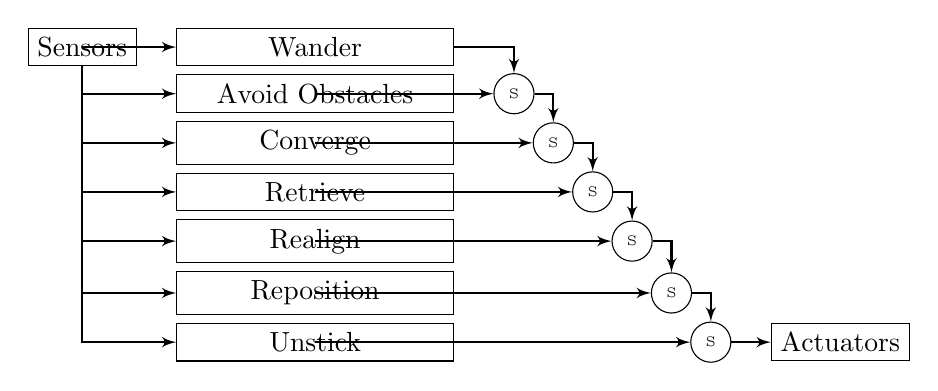
\begin{tikzpicture}

\tikzstyle{behaviour}=[draw, minimum width=10em, right=5mm of sensors]
\tikzstyle{line}=[draw, thick, -latex']
\tikzstyle{subsumption}=[draw, circle]

\node[draw] (sensors) {Sensors};

\node[behaviour] (wander) {Wander};
\node[behaviour, below=1mm of wander] (avoid_obstacles) {Avoid Obstacles};
\node[behaviour, below=1mm of avoid_obstacles] (converge) {Converge};
\node[behaviour, below=1mm of converge] (retrieve) {Retrieve};
\node[behaviour, below=1mm of retrieve] (realign) {Realign};
\node[behaviour, below=1mm of realign] (reposition) {Reposition};
\node[behaviour, below=1mm of reposition] (unstick) {Unstick};


\node[subsumption, right=5mm of avoid_obstacles] (avoid_obstacles_subsumption) {\tiny S};
\node[subsumption, right=10mm of converge] (converge_subsumption) {\tiny S};
\node[subsumption, right=15mm of retrieve] (retrieve_subsumption) {\tiny S};
\node[subsumption, right=20mm of realign] (realign_subsumption) {\tiny S};
\node[subsumption, right=25mm of reposition] (reposition_subsumption) {\tiny S};
\node[subsumption, right=30mm of unstick] (unstick_subsumption) {\tiny S};
\node[draw, right=5mm of unstick_subsumption] (actuators) {Actuators};

\path[line] (sensors) |- (wander);
\path[line] (sensors) |- (avoid_obstacles);
\path[line] (sensors) |- (converge);
\path[line] (sensors) |- (retrieve);
\path[line] (sensors) |- (realign);
\path[line] (sensors) |- (reposition);
\path[line] (sensors) |- (unstick);

\path[line] (avoid_obstacles) |- (avoid_obstacles_subsumption);
\path[line] (converge) |- (converge_subsumption);
\path[line] (retrieve) |- (retrieve_subsumption);
\path[line] (realign) |- (realign_subsumption);
\path[line] (reposition) |- (reposition_subsumption);
\path[line] (unstick) |- (unstick_subsumption);

\path[line] (wander) -| (avoid_obstacles_subsumption);
\path[line] (avoid_obstacles_subsumption) -| (converge_subsumption);
\path[line] (converge_subsumption) -| (retrieve_subsumption);
\path[line] (retrieve_subsumption) -| (realign_subsumption);
\path[line] (realign_subsumption) -| (reposition_subsumption);
\path[line] (reposition_subsumption) -| (unstick_subsumption);
\path[line] (unstick_subsumption) -- (actuators);

\end{tikzpicture}
\caption{The subsumption architecture of Bearded Octoninja.}
\label{figure:subsumption}
\end{figure}


\bibliography{reference-library}
\bibliographystyle{plain}
\nocite{*}

\end{document}
